\chapter{Methodology outtakes}

Sense-making uses various methods including drill-down, covered in \secref{drill-down-research-method}, and various other methods listed here:

\begin{itemize}
\itemsep0em
    \item Drill-down in the current mobile analytics tool for the same app (segment 1 in Figure~\ref{fig:boston-matrix-app-and-mobile-analytics-tool}).
    \item Drill-down in the current mobile tool for other apps (segment 3 in Figure~\ref{fig:boston-matrix-app-and-mobile-analytics-tool}). \\ (If the app incorporates other mobile analytics tools these tools may also help where there is overlapping content common to both tools; for example crashes reported in both Android Vitals and in Crashlytics, (segment 2 in Figure~\ref{fig:boston-matrix-app-and-mobile-analytics-tool}).)
    \item Comparing various analytics artefacts, particularly reports, using various criteria. These comparisons may be within a single mobile analytics tool, or across several mobile analytics tools.
    \item Searching grey data\index{Grey data} and grey literature\index{Grey literature} and cross referencing of materials.
    \item Asking people: for instance colleagues, the developers of the app, the developers of the mobile analytics tool, \textit{etc}.
    \item Experimental `spikes' where a simple,  minimal effort piece of code is written to try out an idea~\footnote{\url{https://en.wikipedia.org/wiki/Spike_(software_development)}}. (These tend to require significant effort so are not likely to be used lightly).
    \item Check development artefacts as these may provide relevant and pertinent information and clues.
\end{itemize}


We also need to consider: does anything generalise beyond a single case?


\subsection{Assessment criteria}~\label{rw-assessment-criteria-topic}
For the purposes of this research there are two key dimensions in much of the research: 1) how grounded the work is in the real-world, and 2) how applicable it is to the real-world of developing mobile apps. Figure \ref{fig:grounded-and-applicable-boxplots} is a sketch of the two dimensions with five example topics. The vertical axis assesses how \emph{grounded in reality} the topic is, and the horizontal axis considers the \emph{applicability} of any findings, conclusions, \emph{etc.} %We will cover these topics shortly, % TODO complete the forward links.
before we do there are several pertinent research topics for general software development that help provide context for developing mobile apps.

\begin{figure}
    \centering
    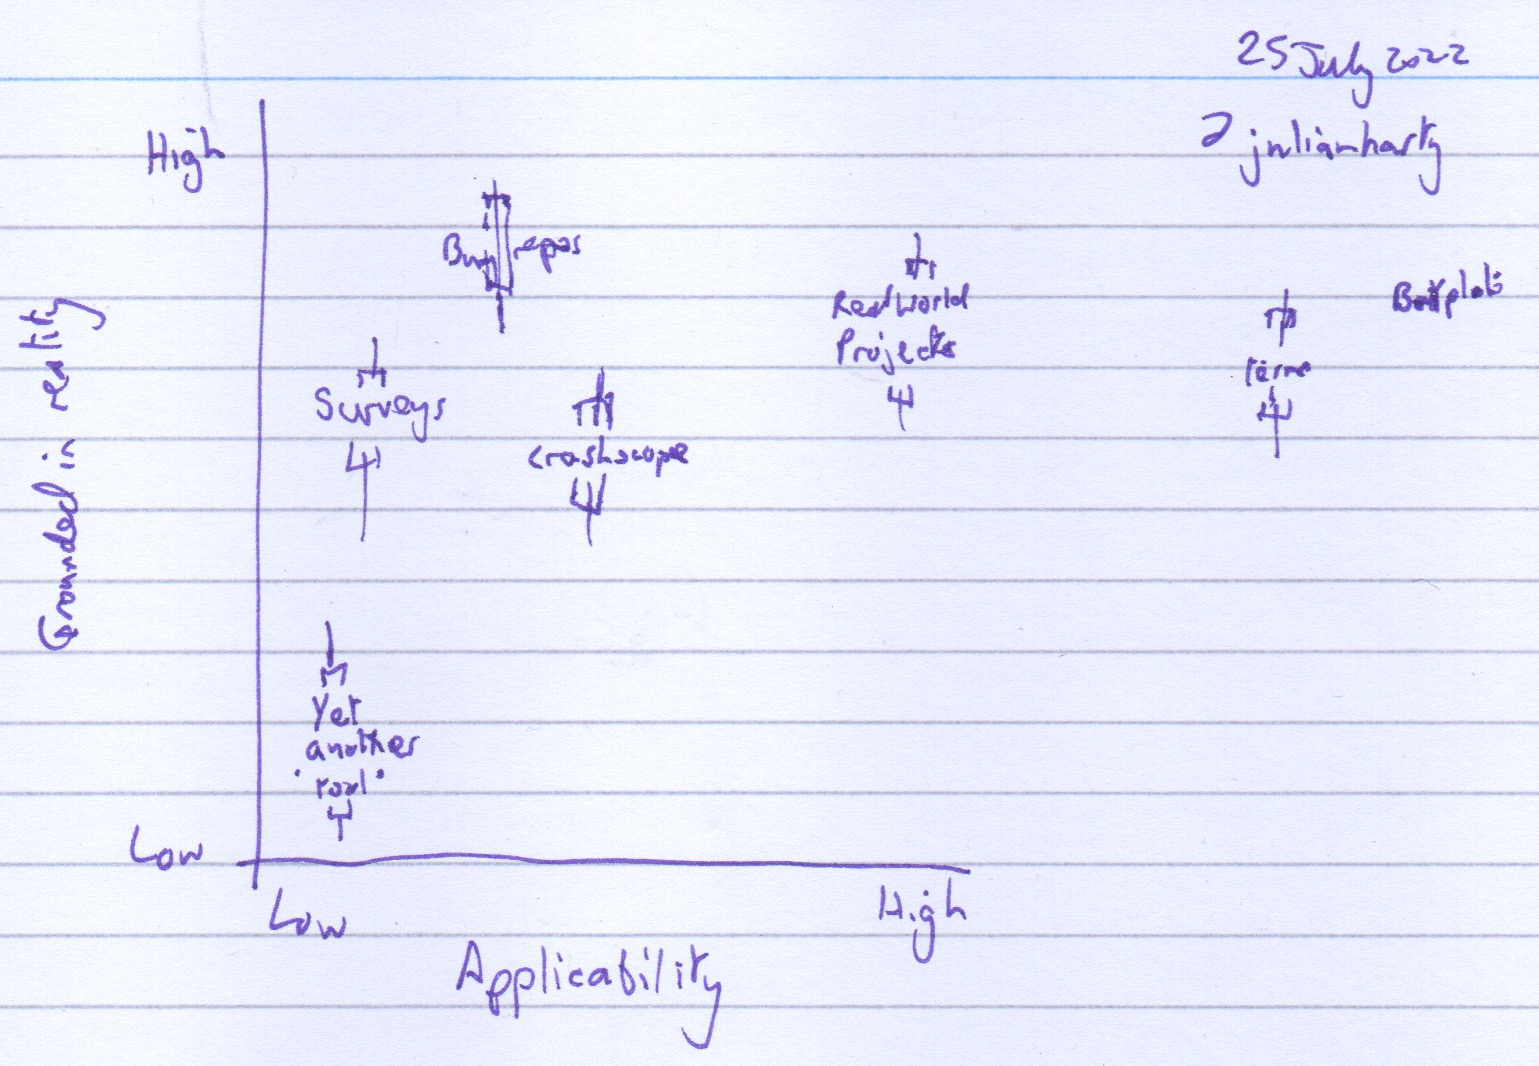
\includegraphics[width=\linewidth]{images/rough-sketches/grounded-and-applicable.jpeg}
    \caption{Box-plots visualising various research in mobile app software development}
    \label{fig:grounded-and-applicable-boxplots}
\end{figure}

